\section{Hourly Marine Heatwave Taxonomy}

\subsection{Taxonomic Framework}

The taxonomic layer is formulated as a set of explicit, event-aligned measurements rather than as a fixed unsupervised classification. This choice preserves interpretability: every descriptor has a declared formula, unit, valid range and implementation. The taxonomy can therefore be expanded as a scientific question changes, while event detection remains stable. Metrics are evaluated over the final event interval and may use raw exceedance, SST, climatology, threshold, temporal indices and spatial coordinates supplied by the rule context.

The current catalogue illustrates complementary dimensions of hourly event structure. Threshold-exceedance fraction quantifies the fraction of valid event hours above the climatological threshold. Daytime strong-exceedance fraction characterises frequent large daytime anomalies relative to the threshold--climatology separation. Heat content integrates positive threshold exceedance through time. Nocturnal below-climatology and below-threshold fractions describe nighttime recovery or interruption. Nocturnal-to-daytime heat retention assesses whether nighttime SST remains above a reference set by the preceding daytime threshold. These descriptors should be interpreted jointly: none is a universal proxy for impact, persistence or cumulative thermal exposure.

\subsection{Feature-Space Representation and Principal Component Analysis}

For multivariate analysis, an event $i$ may be represented as a point in an $N$-dimensional descriptor space,
\[
\mathcal{E}_i = \mathcal{E}\bigl(\tilde{x}_{i1},\tilde{x}_{i2},\ldots,\tilde{x}_{iN}\bigr),
\]
where $x_{ij}$ is the $j$th scalar derived for the event and $\tilde{x}_{ij}$ is its declared normalized form. CUDAHeat returns the raw, physically interpretable scalars; it does not silently normalize descriptors or assign principal components. Normalization is an analysis-stage decision because the appropriate transformation depends on the comparison population, the distribution of each metric and the scientific question. For example, standardization by $\tilde{x}_{ij}=(x_{ij}-\mu_j)/\sigma_j$ is appropriate for principal component analysis (PCA) only when $\mu_j$ and $\sigma_j$ are estimated from a clearly defined event set and variables with zero or near-zero variance are handled explicitly.

PCA can then be applied to the complete, normalized descriptor matrix to identify orthogonal directions of maximal variance. Component scores provide a low-dimensional projection for exploration, whereas loadings identify which standardized descriptors contribute to each component. PCA is descriptive rather than a proof of discrete event types: its interpretation requires reporting the event-selection criteria, transformations, normalization reference set, retained components and explained variance. Missing descriptors should be handled by a declared complete-case or imputation procedure before fitting, rather than being implicitly discarded by plotting software.

\subsection{YAML Rule Catalogues}

Each enrichment rule is a YAML document with a stable identifier, semantic version, short and long names, mathematical formula, symbol definitions, category metadata and output specification. The output specification declares a name, unit, range and dimensions. The rule document also contains a Python \code{calculate} function. At discovery, CUDAHeat validates the schema, rejects duplicate identifiers or output names, compiles the function and records a SHA-256 hash of the source document. This design couples an event variable to its precise mathematical and computational definition.

The explicit formula and symbol metadata are intended to make the taxonomic catalogue suitable for scientific reporting. A rule is not merely a column added to an event table: it is a versioned hypothesis about which aspect of event morphology is informative. The catalogue should consequently be curated with the same care as the detection configuration, including unit consistency, handling of missing values and the physical interpretation of extrema or thresholds.

\subsection{Current Rule Catalogue}

The rule catalogue is presented in Table~\ref{tab:cudaheat-rules}. It is generated directly from the YAML rule specifications in the rule directory and typeset by \code{create_Latex_table.tex}. The catalogue documents the rule symbols, units, formulas, descriptions and interpretations used in the current implementation.

\clearpage
\refstepcounter{table}
\label{tab:cudaheat-rules}
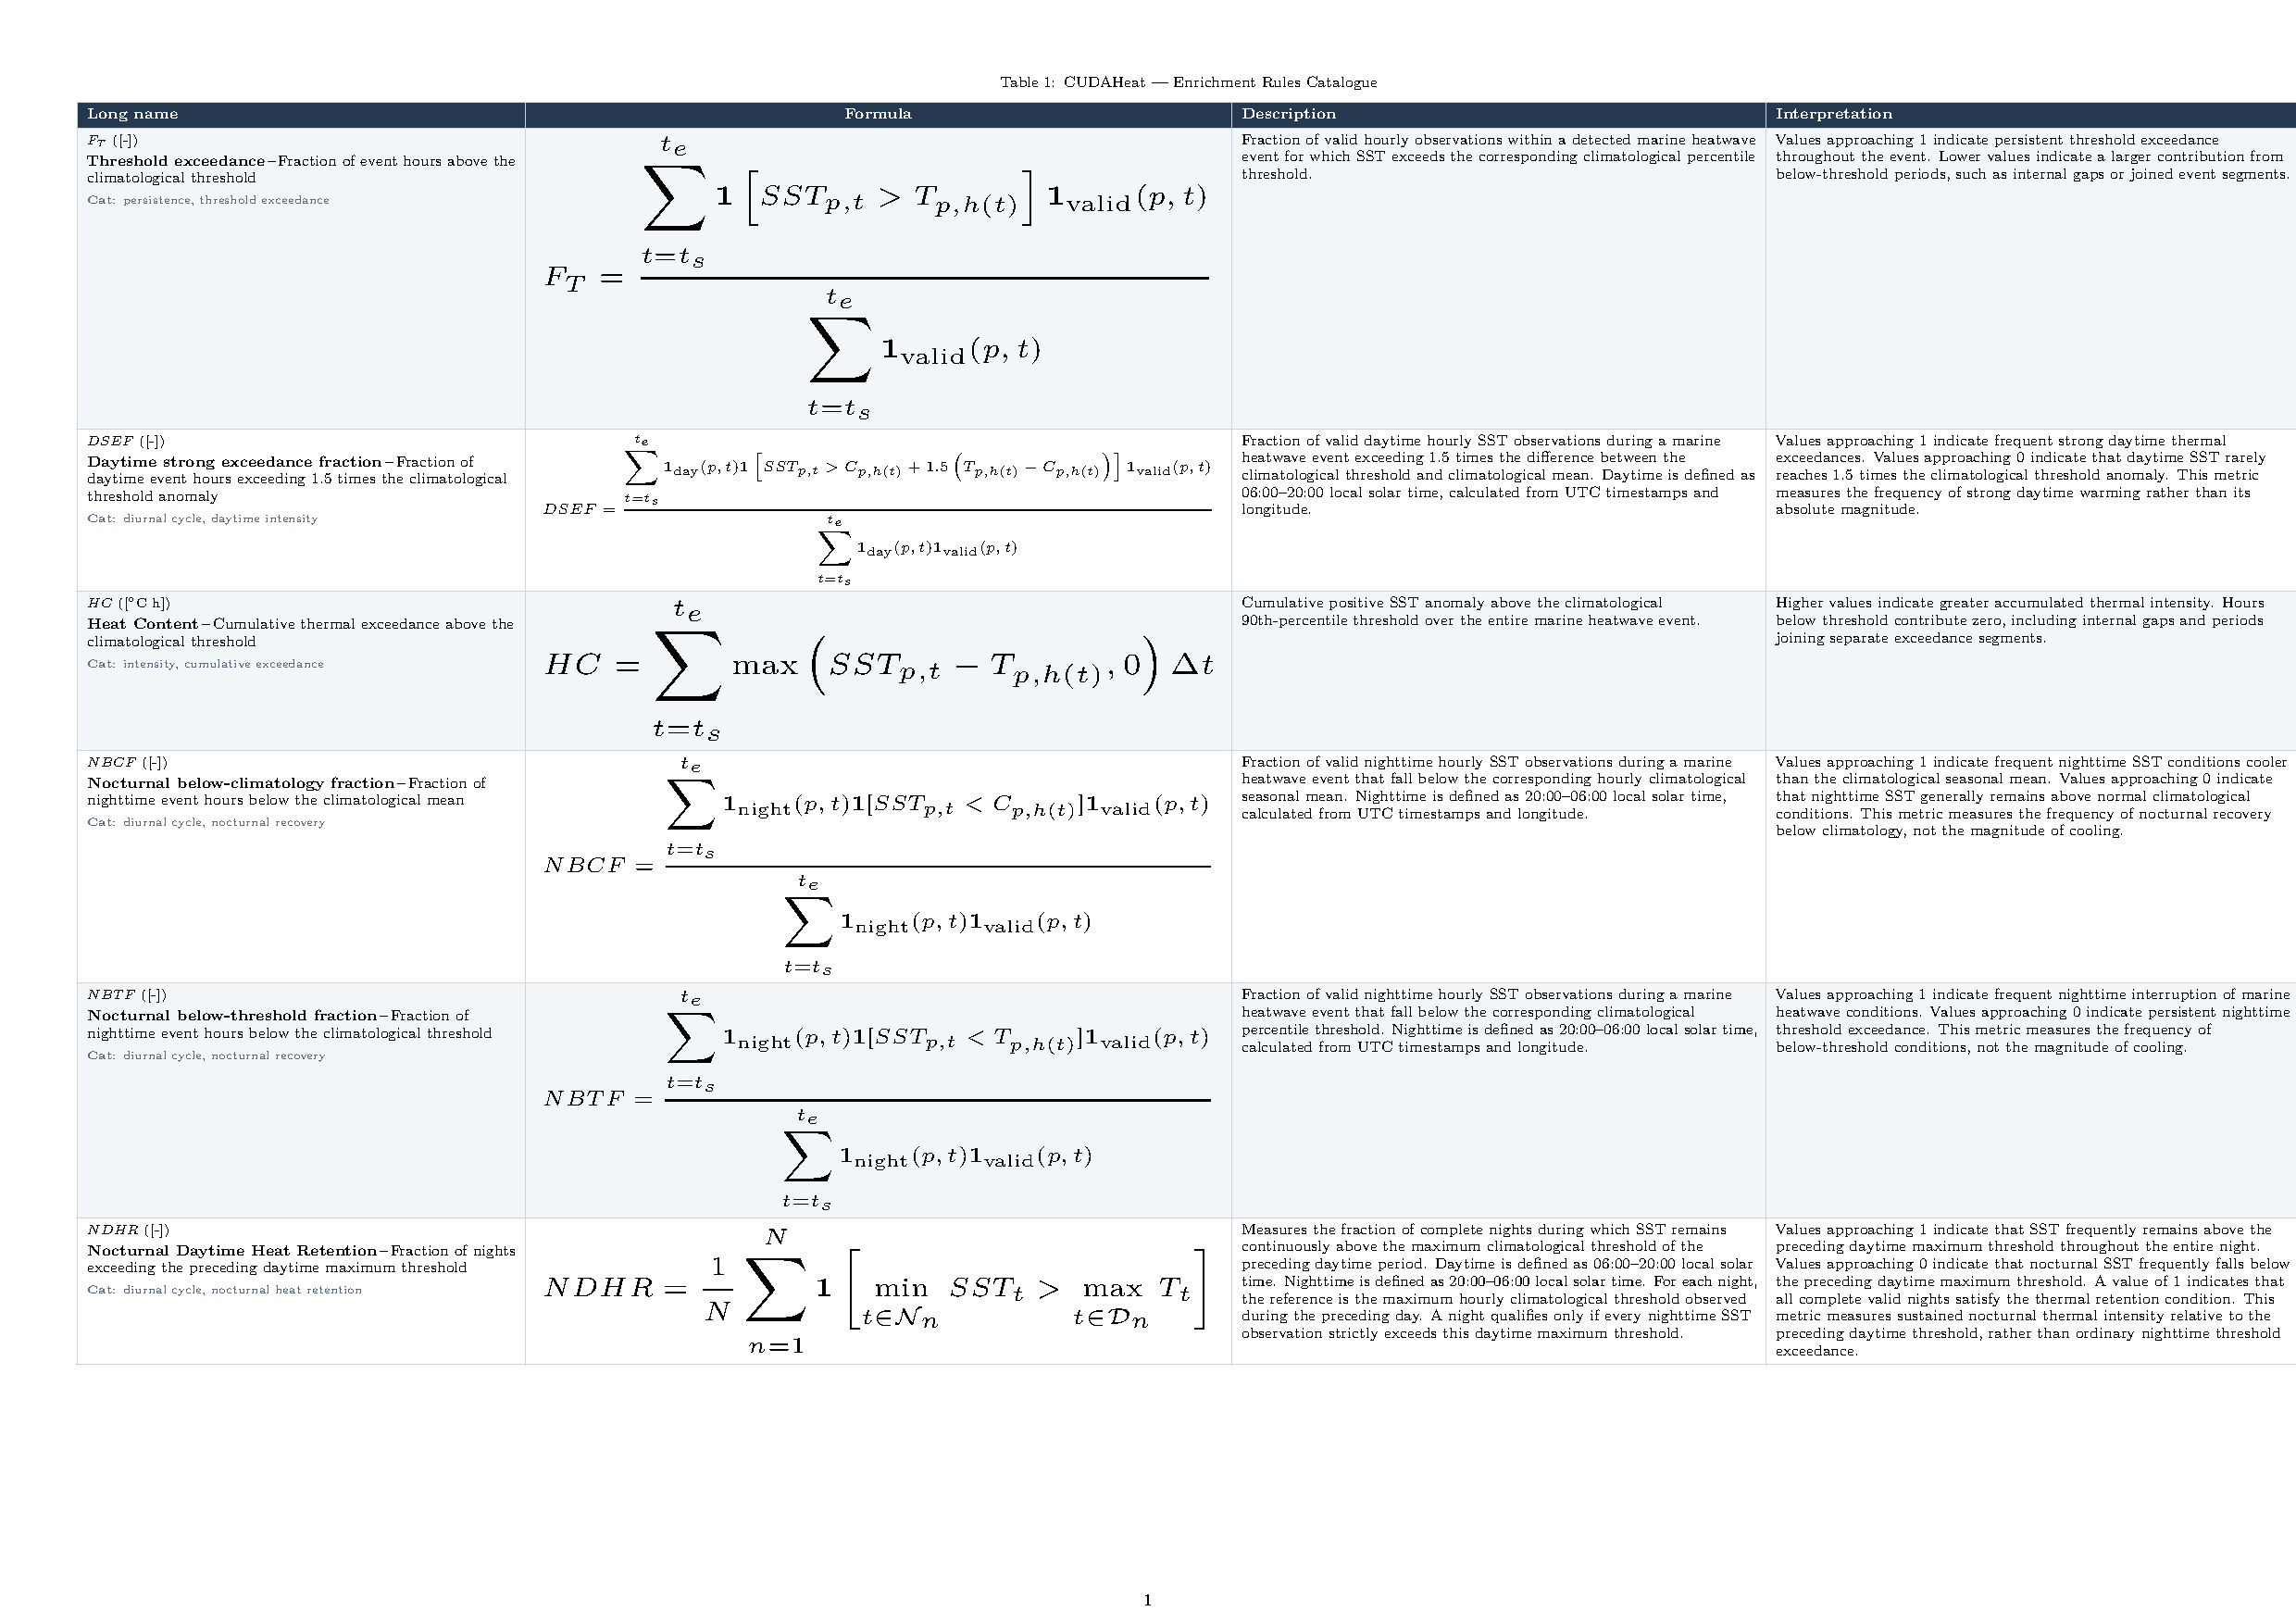
\includepdf[
    pages=-,
    fitpaper=true,
    pagecommand={\thispagestyle{plain}}
]{../examples/rule_laboratory/create_Table/create_Latex_table.pdf}
\clearpage

\subsection{Rule Evaluation}

\noindent\textbf{Integrated and standalone enrichment.}

Integrated enrichment is invoked during \code{detect()} and evaluates rules on device-resident batches after final event intervals have been determined. This avoids a second read of SST and annual-cycle fields. The standalone \code{enrich()} path supports retrospective application of rules to an existing sparse result. It reads the optimized source and cached cycles in storage-local batches, constructs aligned fields only when requested and evaluates interval reductions without iterating over individual events in Python.

Because a YAML rule embeds executable Python, rule directories are trusted extensions of the analysis environment. Schema validation confirms structure and declared metadata; it cannot establish scientific validity or prevent intentional side effects in arbitrary code. Reproducible use therefore requires version control of the rule directory, review of the embedded calculation and preservation of the recorded rule hashes.

\noindent\textbf{Rule provenance and event-aligned outputs.}

Rule outputs are attached to the sparse event catalogue using stable output names. The result metadata records the identifier, version, path, hash, formula and output declaration for every evaluated rule, together with enrichment timing information. This provenance permits a table of event descriptors to be traced back to the exact algorithm and configuration used for its production. It also makes it possible to repeat an enrichment analysis after a rule revision without overwriting or ambiguously merging measurements from different rule versions.
